\section{Data Applications}
\label{sec:applications}

\subsection{Air Quality Sensor Data}
\label{sec:app:spod}

\paragraph{Data.} Our first application revisits the fenceline air-quality monitoring problem that motivated quantile trend filtering in \citet{brantley2020baseline}. The U.S.\ Environmental Protection Agency deploys low-cost SPod sensors on the perimeter of industrial facilities to detect fugitive emissions of volatile organic compounds (VOCs). Each SPod records, once per second, the raw signal of a photoionization detector (PID): a UV lamp ionizes VOC molecules in the sampled air and the resulting current, reported in uncalibrated counts, is proportional to the total concentration of ionizable compounds. The series has three components with sharply different time scales. Emission plumes crossing the sensor produce large one-sided spikes lasting seconds to a few minutes; the electronic baseline drifts slowly over hours with temperature, humidity, and lamp condition; and high-frequency instrument noise rides on top of both. The scientific interest lies exclusively in the spikes, but because each unit's baseline drifts idiosyncratically and the counts are not calibrated across units, the drifting baseline must be estimated and removed before events can be flagged or compared across sensors. Since the plumes are strictly one-sided excursions above the baseline, the baseline is identified by a \emph{low} conditional quantile of the series, making this a natural quantile trend filtering problem in which, in contrast to the usual convention, the trend is the nuisance and the residual carries the signal. We analyze one day of data, June 15, 2018, from sensor \texttt{d} of the two collocated SPods in the EPA Rubbertown dataset accompanying \citet{brantley2020baseline}, aggregating the 86{,}400 raw 1-Hz observations into 10-second block means, which yields $n = 8{,}640$ observations and attenuates the strong serial correlation of the 1-Hz noise that the ALD working likelihood does not model.

\paragraph{Model and settings.} We estimate the baseline at the three levels $\tau \in \{0.01, 0.05, 0.1\}$ with $k = 2$, so the prior favours piecewise quadratic trends, each level fitted independently by the individual sampler of Section~\ref{subsec:individual} on the standardized series. The sampler is run for $6{,}000$ Gibbs iterations with a burn-in of $1{,}000$, proximal parameter $\gamma = 0.1$, smoothing parameter $\epsilon = 0.01$, priors $\lambda \sim \mathrm{Gamma}(1, 10)$ and $\sigma \sim \mathrm{IG}(0.01, 0.01)$, and a step size adapted during burn-in toward acceptance rate $0.5$. Because $S_{D}(\btheta)$ is small for the smooth baselines supported by these data, the rate parameter of the Gamma prior effectively pins the posterior of $\lambda$ near $(n - k - 1)/10 \approx 864$, so the prior acts as a smoothness dial; we return to this point below. As the frequentist benchmark we use the ADMM solver of the \texttt{detrendr} package of \citet{brantley2020baseline} with the smoothing parameter selected by eBIC over the grid $\lambda \in \exp\{-2, \dots, 12\}$, which selects $\lambda = 54.6$ at $\tau = 0.01$ and $\lambda = 1096.6$ at $\tau \in \{0.05, 0.1\}$. Following \citet{brantley2020baseline}, event detection after baseline removal is a threshold rule on the detrended series $\by - \widehat{\btheta}$: a point is classified as signal when it exceeds the empirical 90th, 95th, or 99th percentile of the detrended data themselves, so that no absolute calibration of the counts is required.

\paragraph{Results.} Figure~\ref{fig:spod_quantiles_pmala} overlays the three fitted baselines on the data for the proposed sampler; the corresponding ADMM fits, and the detrended series they produce, are reported in Appendix~\ref{app:spod_admm}. Both methods track the overnight rise, the large morning excursion around 05:00, and the slow afternoon decline, and both leave the plume spikes untouched above the fit. The empirical calibration of the posterior median baselines is close to nominal: the fraction of observations below the fitted curve is $0.005$, $0.044$, and $0.092$ at $\tau = 0.01, 0.05, 0.1$, against $0.000$, $0.043$, and $0.092$ for ADMM. The comparison at $\tau = 0.01$ favours the Bayesian fit: eBIC selects a twenty-fold smaller penalty at this level than at the other two, and the resulting ADMM curve bends upward into the 05:00 plume and crosses the $\tau = 0.05$ and $\tau = 0.1$ curves, whereas the posterior medians, whose smoothness is governed by the same prior at all three levels, remain ordered and essentially parallel throughout the day. Figure~\ref{fig:spod_detrended_pmala} shows the detrended series with the three detection thresholds, and Figure~\ref{fig:spod_detrended_admm} its ADMM counterpart; with the $\tau = 0.05$ baseline removed, the 95\% threshold sits at $109$ counts for the proposed method ($92$ for ADMM) while the largest plumes exceed $400$ counts, so the events of interest separate cleanly from the noise floor under either baseline. Each level required $44$--$53$ minutes of computation at $n = 8{,}640$ ($6{,}000$ iterations), against roughly four minutes for the ADMM fit including the eBIC grid search; acceptance rates were $0.16$, $0.39$, and $0.50$ at $\tau = 0.01, 0.05, 0.1$. Mixing degrades at the most extreme level: the median effective sample size of $\btheta$ is $67$ at $\tau = 0.1$ and $39$ at $\tau = 0.05$, but drops to $3.5$ at $\tau = 0.01$, where fewer than one observation in a hundred lies below the trend and the smoothed check-loss gradient is nearly flat, so pointwise credible statements at $\tau = 0.01$ carry substantial Monte Carlo error at this chain length.

\begin{figure}[htbp]
\centering
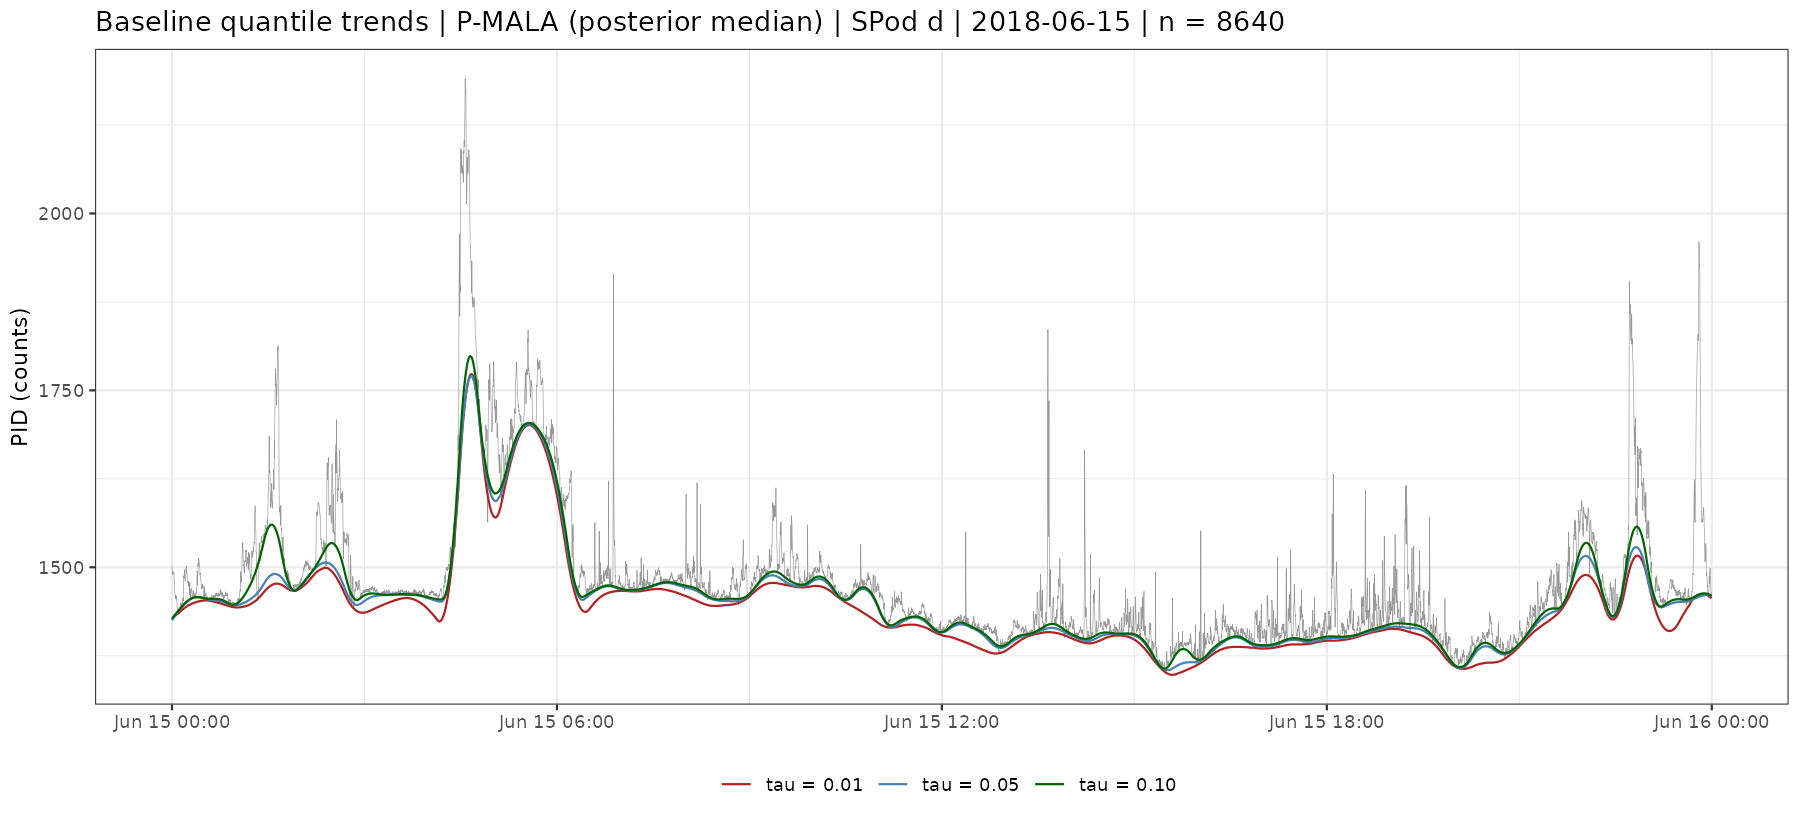
\includegraphics[width=0.75\textwidth]{figures/spod_quantiles_pmala}
\caption{Air quality data: baseline trends at $\tau \in \{0.01, 0.05, 0.1\}$ estimated by the individual P-MALA/Gibbs sampler with $k = 2$ on the 10-second means ($n = 8{,}640$) of SPod \texttt{d}, June 15, 2018. Curves are posterior medians; the grey line is the observed PID series.}
\label{fig:spod_quantiles_pmala}
\end{figure}

\begin{figure}[htbp]
\centering
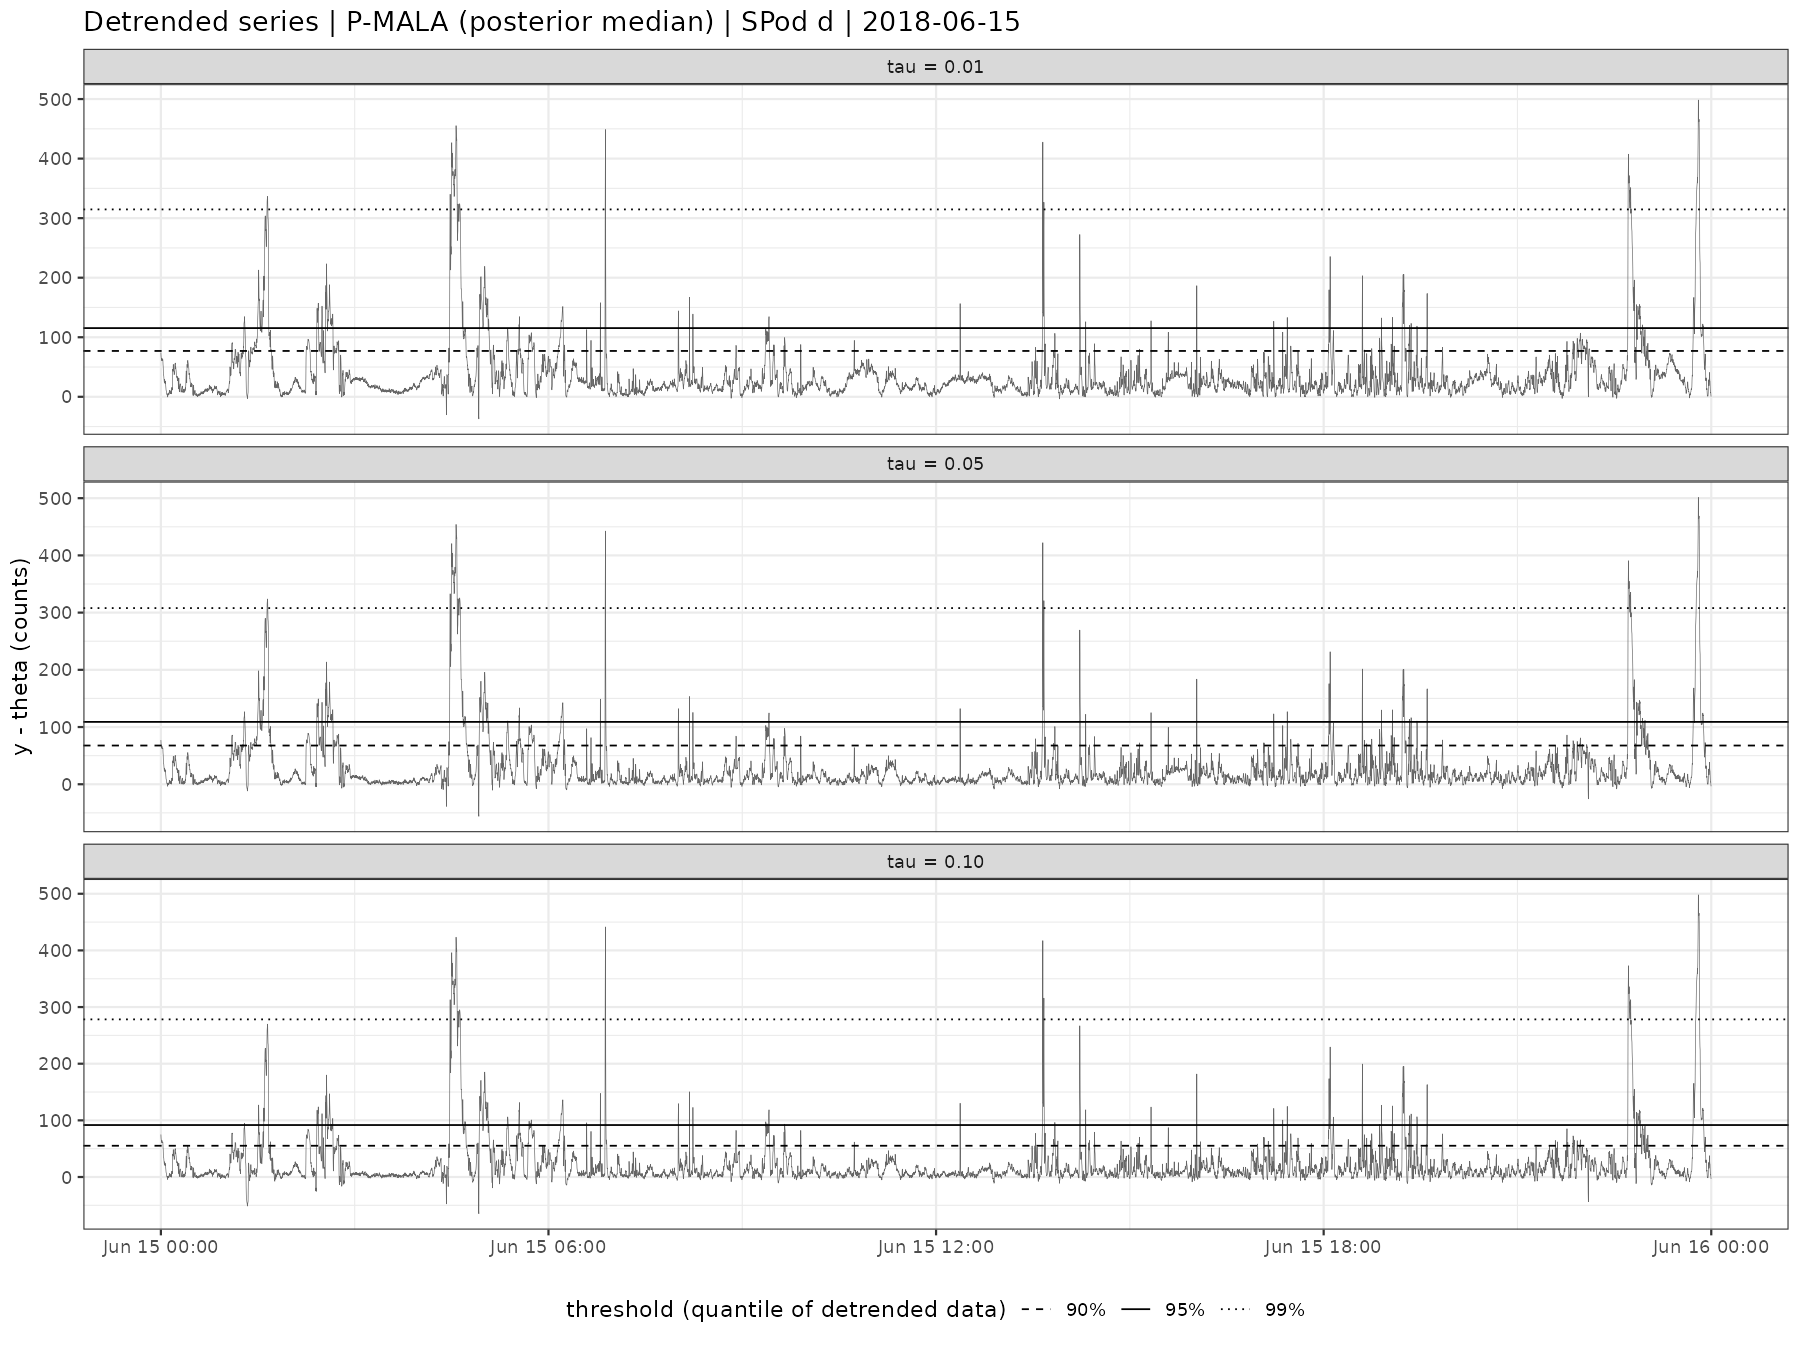
\includegraphics[width=0.75\textwidth]{figures/spod_detrended_pmala}
\caption{Air quality data: detrended series $\by - \widehat{\btheta}$ for the P-MALA baselines of Figure~\ref{fig:spod_quantiles_pmala}, one panel per quantile level. Horizontal lines mark the 90th (dashed), 95th (solid), and 99th (dotted) empirical percentiles of the detrended data, the thresholds used to classify emission events.}
\label{fig:spod_detrended_pmala}
\end{figure}

\subsection{Munich Rent Data}
\label{sec:app:munich}

\paragraph{Data.} The Munich rent data come from the 2003 Munich rental guide (\emph{Mietspiegel}), a survey used by the city to publish reference rents, and are a standard example in the regression literature \citep{fahrmeir2013regression}; they are also the real-data illustration in \citet{onizuka2024fast}, which makes them a natural test bed for comparing the two Bayesian samplers. We use the $N = 2{,}035$ apartments in the version distributed with the \texttt{spmrf} package. The response $y$ is the net rent per square metre (EUR per month) and the covariate $x$ is the floor size in square metres. The design has two features that the simulation study of Section~\ref{sec:simulations} does not exercise. First, floor size is recorded to the square metre, so the $2{,}035$ apartments occupy only $n = 134$ distinct sizes between 17 and 185\,m$^2$, with a median of 13 apartments per size, up to 57 at 65\,m$^2$, and one or two per size above roughly 130\,m$^2$. Second, the observed sizes skip integers, with gaps of up to 5\,m$^2$ in the upper range, so the grid is irregular. The scatter of rent against size (grey circles in Figures~\ref{fig:munich_pmala_1090} and~\ref{fig:munich_onizuka_1090}) shows a steep decline in rent per square metre for small apartments, a long plateau between about 50 and 120\,m$^2$, and a sparse, noisier upper tail.

\paragraph{Model and settings.} Both features are accommodated without changing the samplers. The trend $\theta \in \R^{n}$ is indexed by the $134$ distinct sizes, and the ALD likelihood sums the check loss over all apartments sharing a size, so that each $\theta_j$ is informed by every rent recorded at $x_j$. Unequal spacing enters only through the difference operator: following \citet{onizuka2024fast}, the equally spaced $D^{(k+1)}$ is replaced by the recursively weighted operator $D^{(k+1)} = D^{(1)}\,\mathrm{diag}\{k/(x_{j+k} - x_j)\}\,D^{(k)}$, which reduces to the usual operator when the $x_j$ are equally spaced. We fit $k = 1$, so the prior favours piecewise linear trends in floor size, at the five quantile levels $\tau \in \{0.1, 0.3, 0.5, 0.7, 0.9\}$, each estimated independently by the individual sampler of Section~\ref{subsec:individual}. The sampler is run for $6{,}000$ Gibbs iterations with a burn-in of $1{,}000$, with proximal parameter $\gamma = 0.1$, smoothing parameter $\epsilon = 0.01$, priors $\lambda \sim \mathrm{Gamma}(1,1)$ and $\sigma \sim \mathrm{IG}(0.01, 0.01)$, and a single P-MALA step size $\delta = 0.1$ for all levels, which gives acceptance rates between $0.42$ and $0.61$ across the five levels. As the point of comparison we run the horseshoe sampler of \citet{onizuka2024fast} in MCMC mode using the authors' own code, which handles repeated observations and irregular grids natively, with the same $k$, the same quantile levels, and the same number of iterations and retained draws. For both methods the point estimate is the posterior mean of $\theta$ and the bands are $95\%$ pointwise credible intervals computed from the $5{,}000$ retained draws.

\paragraph{Results.} Figures~\ref{fig:munich_pmala_1090} and~\ref{fig:munich_onizuka_1090} display the fitted $10\%$ and $90\%$ quantile curves, which together bracket the central $80\%$ of the conditional rent distribution at every floor size; in both cases the fraction of rents below each fitted curve matches its nominal level to within $0.005$. The two samplers agree closely over the well-populated range: both place a kink near 42--45\,m$^2$ in the $10\%$ curve, after which the lower quantile is nearly flat at about 5\,EUR/m$^2$, and both show the $90\%$ curve declining gently from about 11 to 9\,EUR/m$^2$ beyond 120\,m$^2$. The visible difference is at the left boundary, where only one or two apartments are observed per size: the horseshoe fit lets the $90\%$ curve rise to about 21\,EUR/m$^2$ at 17\,m$^2$, chasing two isolated high rents, with a correspondingly wide band, whereas the single-scale Laplace prior of the individual sampler keeps it near 14.5\,EUR/m$^2$. The corresponding fits at the interior levels $\tau \in \{0.3, 0.5, 0.7\}$, which are nearly indistinguishable between the two methods, are reported in Appendix~\ref{app:munich_interior}.

\begin{figure}[htbp]
\centering
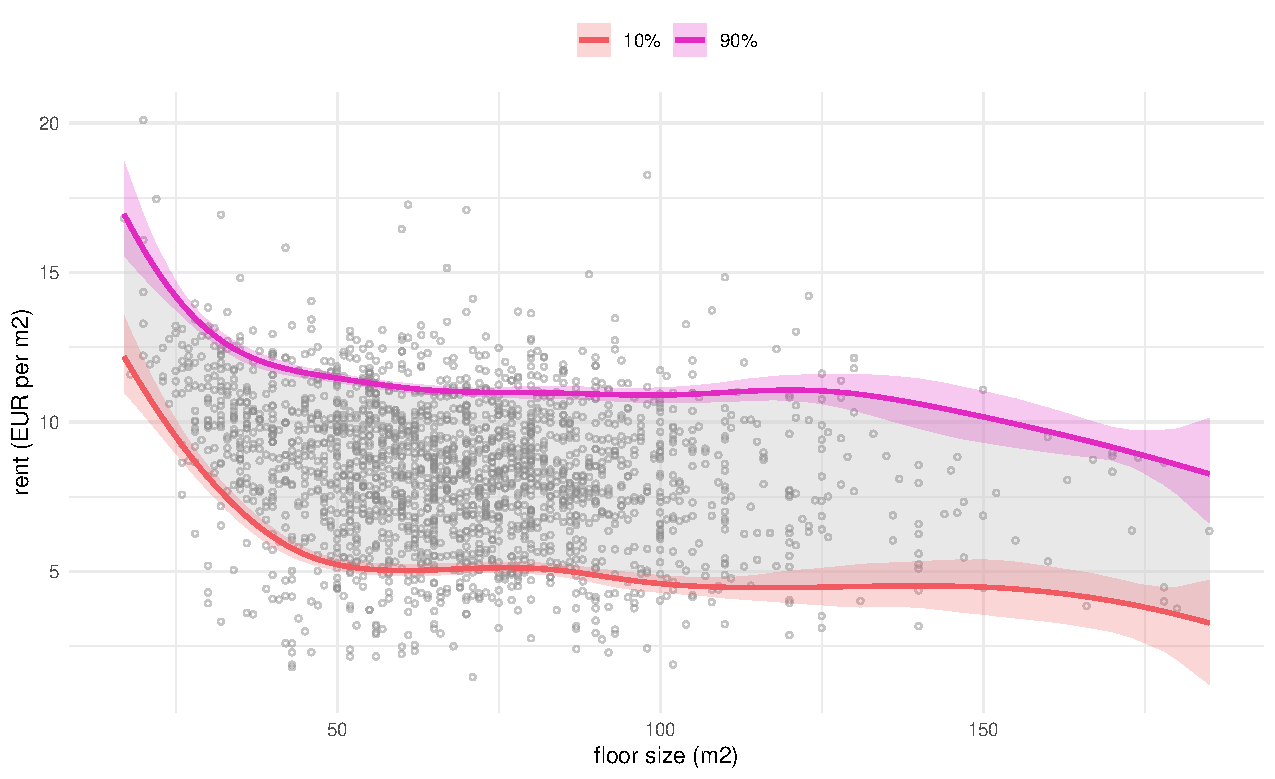
\includegraphics[width=0.75\textwidth]{figures/munich_pmala_q10_q90}
\caption{Munich rent data: $10\%$ and $90\%$ conditional quantiles of rent per square metre as a function of floor size, estimated by the individual P-MALA/Gibbs sampler with $k = 1$. Solid curves are posterior means, coloured ribbons are $95\%$ pointwise credible intervals, and the grey band between the two curves marks the central $80\%$ of the fitted conditional distribution. Grey circles are the $2{,}035$ apartments.}
\label{fig:munich_pmala_1090}
\end{figure}

\begin{figure}[htbp]
\centering
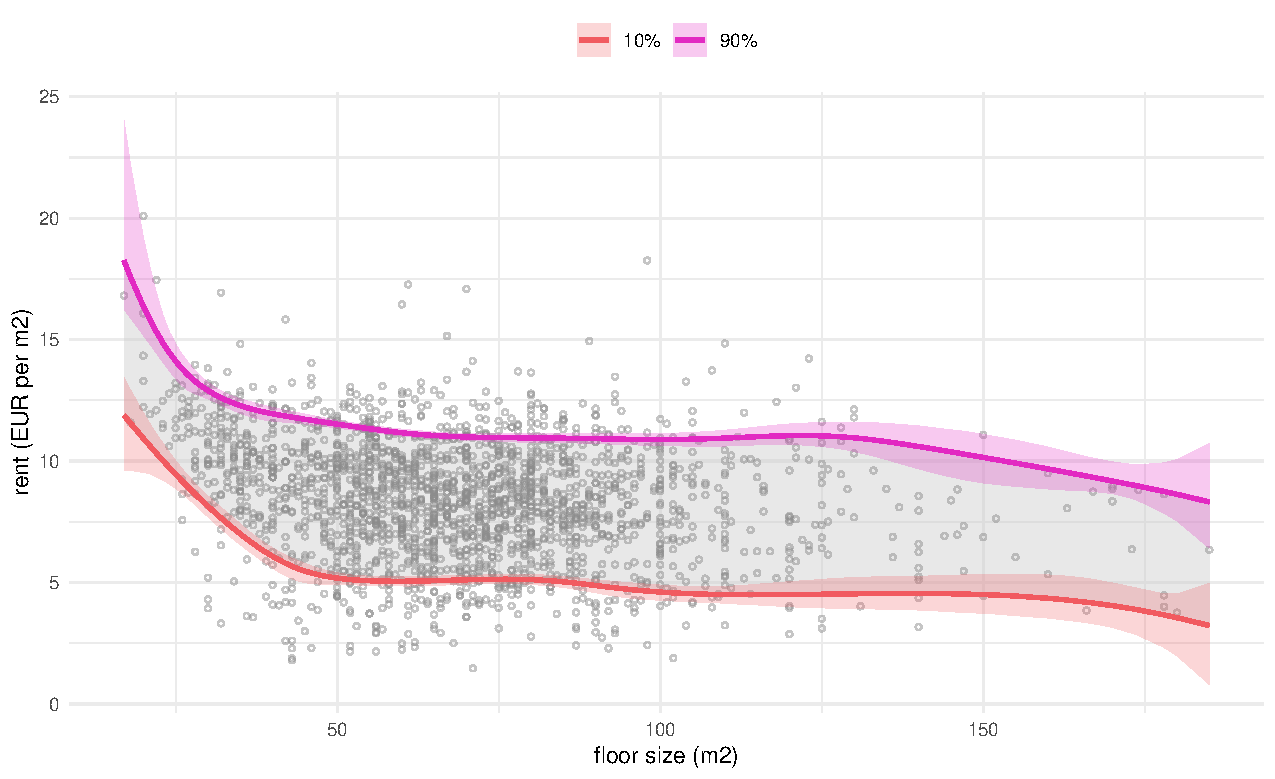
\includegraphics[width=0.75\textwidth]{figures/munich_onizuka_q10_q90}
\caption{Munich rent data: $10\%$ and $90\%$ conditional quantiles estimated by the horseshoe sampler of \citet{onizuka2024fast} (MCMC mode) with $k = 1$, under the same layout as Figure~\ref{fig:munich_pmala_1090}.}
\label{fig:munich_onizuka_1090}
\end{figure}

\subsection{Growth Centiles for Dutch Children}
\label{sec:app:growth}

Growth charts are the canonical use of quantile curves: a child's height is
read against the population centiles at the same age, so the chart itself is a
family of quantile curves indexed by age.  We use the Fifth Dutch Growth Study
\citep{schonbeck2013tallest}, a nationwide cross-sectional sample collected in
2009 and distributed with the \texttt{mice} package
\citep{vanbuuren2011mice}.  After removing records without a height
measurement the data contain 4{,}817 boys and 5{,}190 girls aged 0 to 22
years, each measured once.  Boys and girls are analysed separately.

As with the Munich rents, many children share a covariate value.  We round
age to the nearest tenth of a year, which gives $G = 220$ equally spaced age
slots for boys and $G = 221$ for girls, and index the trend
$\btheta \in \R^{G}$ by slot; the likelihood sums the check loss over all
children in a slot exactly as in Section~\ref{sec:app:munich}, and because
the grid is equally spaced the difference operator needs no reweighting.  We
fit
$k = 2$ with $\lambda \sim \mathrm{Gamma}(1, \sqrt{G})$, one independent run
per level $\tau \in \{0.1, 0.3, 0.5, 0.7, 0.9\}$, each for 6{,}000
iterations with 1{,}000 burn-in, and report the posterior mean.  The
linear-in-$n$ prior of Section~\ref{subsec:individual} is calibrated to one
observation per design point; with some twenty children per slot the
likelihood is far more concentrated, and a prior centred near $2G$ leaves the
P-MALA step unable to move, so we use the $\sqrt{n}$ rule instead.

As a benchmark we fit the LMS method \citep{cole1992smoothing}, the standard
tool for growth references.  At each age, height is assumed to follow a
Box--Cox Cole--Green distribution whose median, coefficient of variation and
Box--Cox power are smooth functions of age; all centiles are read off this one
fitted distribution, so they cannot cross by construction, at the price of a
parametric shape assumption at every age.  We use the \texttt{lms} function
of the \texttt{gamlss} package \citep{rigby2005generalized}.

Figure~\ref{fig:growth_boys} shows the five fitted quantile curves for boys.
The curves follow the fast growth in infancy, the near-linear childhood phase,
the pubertal spurt and the adult plateau, and they fan out with age as the
height distribution widens.  In-sample calibration is close to nominal: the
fraction of boys below the fitted curve is $0.098$, $0.300$, $0.498$, $0.699$
and $0.903$ at $\tau = 0.1, 0.3, 0.5, 0.7, 0.9$.  Although the five fits are
independent and nothing in the individual sampler enforces non-crossing, the
posterior-mean curves for girls never cross, and those for boys cross at a
single grid point (age $0.1$ years, where the $0.5$ and $0.7$ curves invert by
$0.6$~cm), out of $880$ adjacent comparisons.  The girls' fit and the LMS
centiles for both sexes are reported in Appendix~\ref{app:growth}
(Figures~\ref{fig:growth_girls}--\ref{fig:growth_lms_girls}).  The two methods
agree closely between roughly one and eighteen years of age and differ at the
ends of the age range, where few children are observed: the LMS centiles
follow the local data more closely, whereas the trend-filtering curves
extrapolate the piecewise-quadratic trend, sitting slightly above the newborn
measurements and bending at the oldest ages.

\begin{figure}[htbp]
\centering
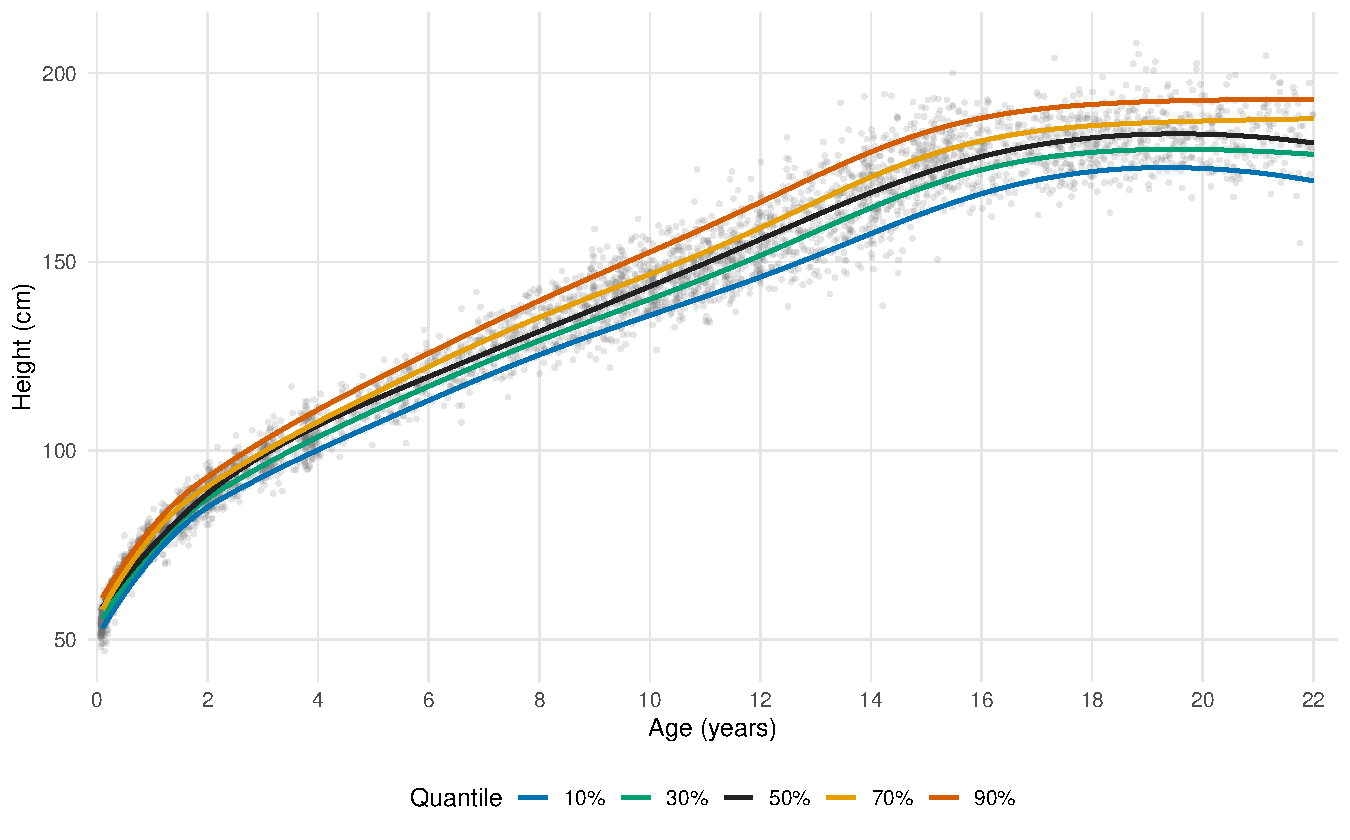
\includegraphics[width=0.75\textwidth]{figures/growth_pmala_boys}
\caption{Individual P-MALA/Gibbs fits for the height of 4{,}817 Dutch boys
(Fifth Dutch Growth Study, 2009) at $\tau \in \{0.1, 0.3, 0.5, 0.7, 0.9\}$,
$k = 2$.  Curves are posterior means on the 0.1-year age grid; grey circles
are the individual measurements.  Each level is fitted independently.}
\label{fig:growth_boys}
\end{figure}


